\documentclass{article}\usepackage[]{graphicx}\usepackage[]{color}
%% maxwidth is the original width if it is less than linewidth
%% otherwise use linewidth (to make sure the graphics do not exceed the margin)
\makeatletter
\def\maxwidth{ %
  \ifdim\Gin@nat@width>\linewidth
    \linewidth
  \else
    \Gin@nat@width
  \fi
}
\makeatother

\definecolor{fgcolor}{rgb}{0.345, 0.345, 0.345}
\newcommand{\hlnum}[1]{\textcolor[rgb]{0.686,0.059,0.569}{#1}}%
\newcommand{\hlstr}[1]{\textcolor[rgb]{0.192,0.494,0.8}{#1}}%
\newcommand{\hlcom}[1]{\textcolor[rgb]{0.678,0.584,0.686}{\textit{#1}}}%
\newcommand{\hlopt}[1]{\textcolor[rgb]{0,0,0}{#1}}%
\newcommand{\hlstd}[1]{\textcolor[rgb]{0.345,0.345,0.345}{#1}}%
\newcommand{\hlkwa}[1]{\textcolor[rgb]{0.161,0.373,0.58}{\textbf{#1}}}%
\newcommand{\hlkwb}[1]{\textcolor[rgb]{0.69,0.353,0.396}{#1}}%
\newcommand{\hlkwc}[1]{\textcolor[rgb]{0.333,0.667,0.333}{#1}}%
\newcommand{\hlkwd}[1]{\textcolor[rgb]{0.737,0.353,0.396}{\textbf{#1}}}%

\usepackage{framed}
\makeatletter
\newenvironment{kframe}{%
 \def\at@end@of@kframe{}%
 \ifinner\ifhmode%
  \def\at@end@of@kframe{\end{minipage}}%
  \begin{minipage}{\columnwidth}%
 \fi\fi%
 \def\FrameCommand##1{\hskip\@totalleftmargin \hskip-\fboxsep
 \colorbox{shadecolor}{##1}\hskip-\fboxsep
     % There is no \\@totalrightmargin, so:
     \hskip-\linewidth \hskip-\@totalleftmargin \hskip\columnwidth}%
 \MakeFramed {\advance\hsize-\width
   \@totalleftmargin\z@ \linewidth\hsize
   \@setminipage}}%
 {\par\unskip\endMakeFramed%
 \at@end@of@kframe}
\makeatother

\definecolor{shadecolor}{rgb}{.97, .97, .97}
\definecolor{messagecolor}{rgb}{0, 0, 0}
\definecolor{warningcolor}{rgb}{1, 0, 1}
\definecolor{errorcolor}{rgb}{1, 0, 0}
\newenvironment{knitrout}{}{} % an empty environment to be redefined in TeX

\usepackage{alltt}

%load packages
\usepackage{tabu}
\usepackage{amssymb, amsmath, amsthm}
\usepackage{enumerate}
\usepackage{geometry}

%no indenting of paragraphs
\setlength{\parindent}{0pt} 


%custom margins
\geometry{top=1.5in, bottom=1.0in, left=1.0in, right=1.0in}

%specify space between paragraphs
\setlength{\parskip}{6pt}

\usepackage{geometry}
\geometry{letterpaper}                   
\usepackage{graphicx}
\usepackage{amssymb}
\usepackage{epstopdf}
\usepackage{amsmath}

\renewcommand{\baselinestretch}{1.}
%\setcounter{page}{0} \thispagestyle{empty}

\setlength{\topmargin}{-0.60in} \setlength{\oddsidemargin}{-0.2in}
\setlength{\textwidth}{6.5in} \setlength{\textheight}{9in}


\def\E{{\rm E}}
\def\T{{\top}}

\def\Var{{\rm Var}}
\def\Cov{{\rm Cov}}
\def\Corr{{\rm Corr}}
\newcommand{\var}{{\rm Var}}

\def\A{\tilde{A}}
\def\a{\tilde{a}}
\def\S{{\rm SWP}}
\def\G{{\rm GJ}}
\def\X{{\bf X}}
\def\Y{{\bf Y}}
\def\Z{{\bf Z}}
\def\R{{\bf R}}
\def\I{{\bf I}}

\def\bbeta{\boldmath{\beta}}

\title{A  Note on Statistical Computing}
\author{Ying Nian Wu, UCLA Statistics}
\date{For STATS 202A, Fall quarter 2017 }
 
\begin{document}
 
\maketitle
 
\tableofcontents
 

\section*{Preface}

This note is mainly about the computational side of the commonly used modern statistical and machine learning methods. The main theme of the first three chapters is linear regression and its rich variations that span much of statistics and machine learning. The last chapter is on Monte Carlo methods. 

Writing R and Python code to implement these methods enable us to gain first-hand experiences with these methods. 

\section{Linear regression: least squares, ridge, Lasso} 

\subsection{Linear Regression}

The dataset of linear regression consists of an $n \times p$ matrix $\X = (x_{ij})$, and a $n \times 1$ vector $\Y = (y_i)$.  The model is of the following form: 
\[
    y_i = \sum_{j = 1}^{p} x_{ij} \beta_j + \epsilon_i,
\]
for $i = 1, ..., n$, where $\epsilon_i \sim {\rm N}(0, \sigma^2)$ independently for $i = 1, ..., n$. Here we are deliberately ambiguous about intercept term. If $x_{i1} = 1$ for all $i$, then $\beta_1$ will be the the intercept term. $[\X, \Y]$ is called the training data. $y_i$ is called response variable, outcome, dependent variable. $x_{ij}$ is called predictor, regressor, covariate, independent variable, or simple variable. In the experimental design setting, $\X$ is called the design matrix. 

\begin{table}[h]
\centering
\begin{tabular}{|c|c|c|}
\hline
 obs & $\X_{n\times p}$ & $\Y_{n\times 1}$ \\
\hline\hline
 1   & $x_{11}, x_{12}, ..., x_{1p}$         & $y_1$ \\
 2   & $x_{21}, x_{22}, ..., x_{2p}$         & $y_2$ \\
...  &                 &\\
$n$  &  $x_{n1}, x_{n2}, ..., x_{np}$        & $y_n$ \\
\hline
\end{tabular}
\end{table}

The process of estimating $\beta$ is called learning from the training data. The purpose is two-fold. 

(1) Explanation: understanding the relationship between $y_i$ and $(x_{ij}, j = 1, ..., p)$. 

(2) Prediction: learn to predict $y_i$ based on $(x_{ij}, j = 1, ..., p)$, so that in the testing stage, if we are given the predictor variables, we should be able to predict the outcome. 


\begin{table}[h]
\centering
\begin{tabular}{|c|c|c|}
\hline
 obs & $\X_{n\times p}$ & $\Y_{n\times 1}$ \\
\hline\hline
 1   & $X_1^\T$         & $y_1$ \\
 2   & $X_2^\T$         & $y_2$ \\
...  &                 &\\
$n$  &  $X_n^\T$        & $y_n$ \\
\hline
\end{tabular}
\end{table}

We can arrange the data in terms of $X_i^\T = (x_{ij}, j = 1, ..., p)$, where $X_i^\T$ is the $i$-th row of $\X$ . Here $X_i$ is not in bold font.  We can write the model as $y_i = X_i^\T \beta + \epsilon_i$, where $\bbeta = (\beta_{j}, j = 1, ..., p)^\T$.

\begin{table}[h]
\centering
\begin{tabular}{|c|c|c|}
\hline
 obs & $\X_{n\times p}$ & $\Y_{n\times 1}$ \\
\hline\hline
$\begin{matrix} 1\\ 2\\...\\ n \end{matrix}$  & $\X_1, \X_2, ..., \X_p$         & $\Y$ \\
\hline
\end{tabular}
\end{table}

We can also arrange the data in terms of $\X_j = (x_{ij}, i = 1, ..., n)$, where $\X_j$ is the $j$-th column of $\X$. Here $\X_j$ is in bold font.  We can write the model as $\Y = \sum_{j=1}^{p} \X_j \beta_j + \epsilon$, where $\epsilon = (\epsilon_i, i = 1, ..., n)^\T \sim {\rm N} (0, \sigma^2 \I_n)$, where $\I_n$ is the $n$-dimensional identity matrix. 

We can write the linear regression model as $\Y = \X^{\T}\bbeta + \epsilon$. The least squares estimate of $\beta$ is 
\[
\hat{\beta} = \arg\min_{\beta} \|\Y - \X\bbeta\|_{\ell_2}^{2} = (\X^{\T}\X)^{-1}\X^{\T}\Y.
\]
We construct a matrix $\Z = [\X  \Y]$, and let 
$$A= \Z^{\T}\Z = \begin{bmatrix} \X^{\T}\X & \X^{\T}\Y \\ \Y^{\T}\X & \Y^{\T}\Y \end{bmatrix}$$ 
be the cross-product matrix. Then 
\[\S[1:p]A = \begin{bmatrix} -(\X^{\T}\X)^{-1} & (\X^{\T}\X)^{-1}\X^{\T}\Y \\ \Y^{\T}\X(\X^{\T}\X)^{-1} & \Y^{\T}\Y - \Y^{\T}\X(\X^{\T}\X)^{-1}\X^{\T}\Y \end{bmatrix} = \begin{bmatrix} -\dfrac{\Var(\hat{\beta})}{\sigma^2} & \hat{\beta} \\ \hat{\beta}^{\T} & \textrm{RSS} \end{bmatrix},\]
where $\textrm{RSS} = \|\Y - \X\hat{\beta}\|_{\ell_2}^2$  is the residual sum of squares. 

We shall expand our treatment of linear regression in later sections. For now, it is enough to know that the sweep operator gives us all the key results we need for linear regression. 


\subsection{Gauss-Jordan elimination} 

For a system of linear equations $A x = b$, where $A = (a_{ij})$ is $n \times n$, $x = (x_i)$ is $n \times 1$, and $b  = (b_i)$ is $n \times 1$, we can solve $x = A^{-1} b$ by Gauss-Jordan elimination. 

Specifically, for any matrix $A$ (here we assume $A$ can be any $n \times N$ matrix, e.g., $N = n+1$ or $N = 2n$), let $\A = \G[k] A$, then 
\begin{eqnarray*} 
   \A_{k} &=& A_k/a_{kk}, \\
   \A_{i} &=& A_i - a_{ik} \A_k, \; i \neq k,
\end{eqnarray*}
where $A_k$ is the $k$-th row of $A$. The above operation makes $\a_{kk} = 1$, and $\a_{ik} = 0$ for $i \neq k$. We can apply Gauss-Jordan sequentially, e.g., $\G[1:m]$ means we apply  Gauss-Jordan  for $k = 1: m$. Being a row operation, Gauss-Jordan is linear, i.e., $\A = \G[k] A$ amounts to $\A = G_k A$ for a matrix $G_k$. Thus 
\[
\G[1:n][A|b]= [I| A^{-1}b ]= A^{-1}[A|b],  
\]
\[
\G[1:n] [A|I] = [I | A^{-1}]= A^{-1}[A|I].  
\]
That is, $\G[1:n] = A^{-1}$, and order does not matter. Moreover, 
\[
   \G[1:m]  \begin{bmatrix} A_{11} & A_{12} & | & I_1 & 0 \\ A_{21} & A_{22} & | & 0 & I_2 \end{bmatrix} = 
   \begin{bmatrix} I_1 & A_{11}^{-1} A_{12} & | & A_{11}^{-1} & 0 \\ 0& A_{22} - A_{21} A_{11}^{-1} A_{12} & | & - A_{21} A_{11}^{-1} & I_2 \end{bmatrix} . 
\]
We can write $\G[1:m] = \G[A_{11}]$, which is a matrix version of Gauss-Jordan. If we compare Gauss-Jordan $\G[1:m]$ with the sweep operator $\S[1:m]$, we can see that sweep operator is a space saving version of Gauss-Jordan, where we do not record the identity matrix in sweep. Because $\G[1:m] = \G[A_{11}]$, we have $\S[1:m] = \S[A_{11}]$. The above equation also leads to the identity 
\[
    |A| = |A_{11}||A_{22} - A_{21} A_{11}^{-1} A_{12}|, 
 \]
 where $|A|$ denotes the determinant of $A$. Thus we can compute $|A|$ by the sweep operator, in addition to $A^{-1}$. 

\subsection{Calculation details} 

To flesh out the details of least squares estimation, let 
\[
    R(\beta) = \sum_{i=1}^{n} \left(y_i - \sum_{j=1}^{p} x_{ij} \beta_j\right)^2, 
  \]
  we have 
  \[
     \frac{R(\beta)}{\partial \beta_j}  = -2 \sum_{i=1}^{n} \left(y_i - \sum_{j=1}^{p} x_{ij} \beta_j\right) x_{ij}. 
  \]
  We can pack the above results in terms of $\X_j$ and $X_i$. Recall 
  \begin{table}[h]
\centering
\begin{tabular}{|c|c|c|}
\hline
 obs & $\X_{n\times p}$ & $\Y_{n\times 1}$ \\
\hline\hline
 1   & $X_1^\T$         & $y_1$ \\
 2   & $X_2^\T$         & $y_2$ \\
...  &                 &\\
$n$  &  $X_n^\T$        & $y_n$ \\
\hline
\end{tabular}
\end{table}

\begin{table}[h]
\centering
\begin{tabular}{|c|c|c|}
\hline
 obs & $\X_{n\times p}$ & $\Y_{n\times 1}$ \\
\hline\hline
$\begin{matrix} 1\\ 2\\...\\ n \end{matrix}$  & $\X_1, \X_2, ..., \X_p$         & $\Y$ \\
\hline
\end{tabular}
\end{table}

    \[
     \frac{\partial R(\beta)}{\partial \beta_j}  = -2 \langle \Y - \sum_{j=1}^{p} \X_j \beta_j, \X_j\rangle = -2 \X_j^\T ( \Y - \sum_{j=1}^{p} \X_j \beta_j), 
  \]
  \[
     R'(\beta) = \begin{bmatrix} \partial R/\partial \beta_1\\ \partial R/\partial \beta_2 \\ ...\\ \partial R/\partial \beta_n \end{bmatrix} = 
      -2 \sum_{i=1}^{n} \left(y_i - \sum_{j=1}^{p} x_{ij} \beta_j\right)  \begin{bmatrix} x_{i1}\\ x_{i2}\\ ... \\x_{ip} \end{bmatrix} 
      = - 2\sum_{i=1}^{n} (y_i - X_i^\T\beta) X_i. 
     \]
We can further pack the above two equations as 
    \[
     \frac{\partial R(\beta)}{\partial \beta_j}  = -2  \X^\T ( \Y - \X\beta). 
  \]
For the second derivative, 
   \[
     \frac{\partial^2 R(\beta)}{\partial \beta_j \beta_k}  = 2 \sum_{i=1}^{n} x_{ij} x_{ik} = 2 \langle \X_j, \X_k\rangle. 
  \]
  Define 
  \[
  R''(\beta) = \left(      \frac{\partial^2 R(\beta)}{\partial \beta_j \beta_k}  \right) 
  \]
  be the $p\times p$ matrix, we can write 
 \[
    R''(\beta) = 2\sum_{i=1}^{n} X_i X_i^\T =  2 \X^\T \X, 
    \]
    which is positive definite. 
    
In order to solve the least squares problem, we only need to solve $R'(\beta) = 0$. Geometrically, it means $\X_j \perp \R$, where $\R  = \Y -\hat{\Y}$, and  $\hat{\Y} =  \sum_{j=1}^{p} \X_j \hat{\beta}_j$ is the projection of $\Y$ onto the subspace spanned by $(\X_j, j = 1, ..., p)$. 

\begin{figure}[h]
\centering
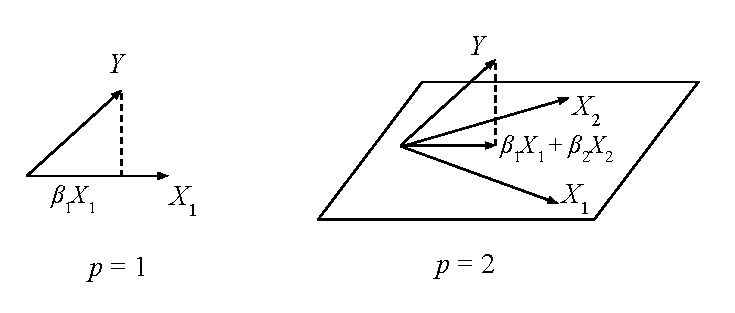
\includegraphics[width=0.5\linewidth]{figures/least-squares.pdf}
\caption{Least squares projection}
\end{figure}

The calculation for ridge regression is similar. Let $f(\beta) = \|\Y  - \X\beta\|_{\ell_2}^2 + \lambda \|\beta\|_{\ell_2}^2$, then 
\[
f'(\beta) = -2 \X^\T(\Y-\X\beta) + 2 \lambda \beta,
\]  
\[
f''(\beta)  = 2 (\X^\T \X + \lambda \I_p). 
\]

\subsection{Matrix calculus} 

Suppose $Y = (y_i)_{m \times 1}$, and $X = (x_j)_{n \times 1}$. Suppose $Y = h(X)$.  We can define 
\[
\frac{\partial Y}{\partial X^\T} = \left(\frac{\partial y_i}{\partial x_j}\right)_{m\times n}.
\]
 If $Y$ is a scaler, then the gradient $h'(X) = \partial Y/\partial X$ is a $n\times 1$ column vector, and $\partial Y/\partial X^\T$ is a $1 \times n$ row vector. For scaler $Y$, we can define the Hessian or second derivative 
 \[
h''(X) = \frac{ \partial^2Y}{\partial X \partial X^\T} = \left(\frac{\partial^2 Y}{\partial x_i \partial x_j}\right)_{n \times n}.
 \] 
If $Y = AX$, then $y_i = \sum_{k} a_{ik} x_k$. Thus $\partial y_i/\partial x_j = a_{ij}$. So $\partial Y / \partial X^\T = A$. 

{\em Chain rule}. If $Y = h(X)$ and $X = g(Z)$, then $\partial y_i/\partial z_j = \sum_k (\partial y_i/\partial x_k)(\partial x_k/\partial z_j)$. Thus 
\[
\frac{\partial Y}{ \partial Z^\T} = \frac{\partial Y}{ \partial x^\T}\frac{\partial X}{ \partial Z^\T}.
\]

{\em Product rule}. If $Y = \langle h(X), g(X)\rangle = \sum_i h_i(X) g_i(X)$, then $\partial Y/\partial x_j = \sum_i [\partial h_i/\partial x_j g_i + h_i  \partial g_i/\partial x_j] $. So 
\[
\frac{\partial Y}{\partial X^\T} = h(X)^\T \frac{\partial g(X)}{\partial X^\T} + g(X)^\T \frac{\partial h(X)}{\partial X^\T}.
\] 

{\em Taylor expansion}
\[
f(X) = f(X_0) + \langle f'(X_0), X-X_0\rangle + \frac{1}{2} (X-X_0)^\T f''(X_0) (X-X_0) + o(|X-X_0|^2).
\] 
	
{\em Jacobian}. Let $Y = h(X)$ where both $X$ and $Y$ are $n \times 1$. Assume that $h$ is one-to-one differentiable mapping.  Let $D_X$ be a local region around $X$ in the domain of $X$. Suppose $h$ maps $D_X$ to a region $D_Y$ in the domain of $Y$. Then as the size of $D_X$ goes to 0, $|D_Y|/|D_X| \rightarrow |h'(X)|$, where $|h'(X)|$ is the determinant of $h'(X) = \partial Y/\partial X^\T$. 


For $R(\beta) = \|\Y - \X\beta\|^2$, $R'(\beta) = - 2 \X^{\T} (\Y - \X\beta)$ and $R''(\beta) = 2 \X^\T \X$. We can derive these by the chain rule. Let $e = \Y - \X \beta$. Then 
\[
   \frac{\partial R}{\partial \beta^\T} = \frac{\partial R}{\partial e^\T} \frac{\partial e}{\partial \beta^\T} = -2 e^\T \X. 
\]
$R'(\beta) = \partial R/\partial \beta$, which is obtained by transposing $-2 e^\T \X$.  
\[
R''(\beta) =\frac{ \partial^2 R}{\partial \beta \partial \beta^\T} = \partial (-2 \X^\T e)/\partial \beta^\T = -  2 \X^\T \X. 
\]


\end{document}
